\documentclass{tmr}

\usepackage{mflogo}
\usepackage{graphicx}
\usepackage{ifpdf}

\title{Hoogle Overview}
\author{Neil Mitchell\email{ndmitchell@gmail.com}}

\begin{document}

\begin{introduction}
This article gives an overview of the Hoogle tool. We describe the history of Hoogle, the improvements that have been made this summer, and plans for future features. Finally, we discuss the design guidelines of Hoogle 4 -- which may be of interest both to budding Hoogle developers and other Haskell projects. This article does not cover the theoretical background of Hoogle.
\end{introduction}

\section{Introduction}

To quote from the Cabal description:

\begin{quote}
``Hoogle is a Haskell API search engine, which allows you to search many standard Haskell libraries by either function name, or by approximate type signature.''
\end{quote}

To explore what Hoogle is, and how it can be used, let's expand on some of those phrases:

\begin{description}
\item[Haskell] Hoogle is written in Haskell, and is designed for Haskell programmers.
\item[search engine] Hoogle is a tool for searching, in a similar vein to Google. \footnote{Hoogle has no affiliation to Google, and the name is intended as a homage.}
\item[API] Hoogle searches with API's, or ``Application Programmer Interfaces'' -- the types and functions provided by a package.
\item[standard libraries] By default, Hoogle will search the libraries that are shipped with most Haskell compilers. These libraries include the base, array, time, mtl etc.
\item[function name] Searches can be performed by name, searching for substrings of function names. One use of Hoogle is as a fast index into Haddock documentation.
\item[type signature] Searches can be performed by type signature, searching for functions of the appropriate type.
\item[approximate] Hoogle tries to find the results you want, even if they don't quite match your actual search.
\end{description}

\begin{figure}
\ifpdf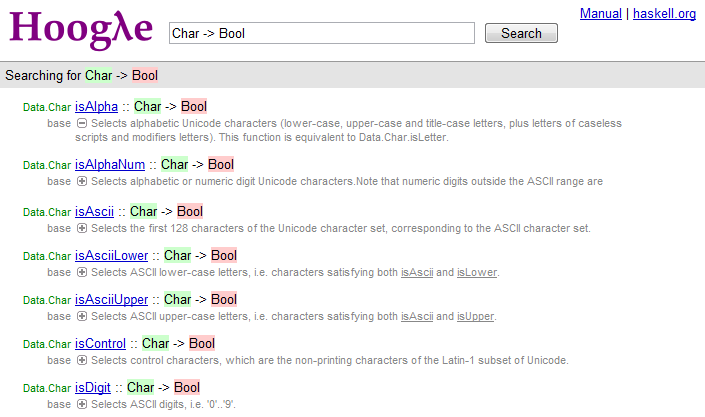
\includegraphics[width=\textwidth]{web.png}\fi
\label{fig:web}
\caption{Hoogle web use.}
\end{figure}

\begin{figure}
\ifpdf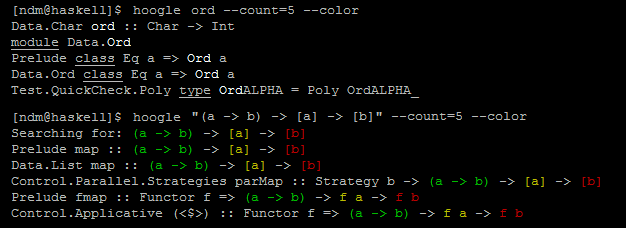
\includegraphics[width=\textwidth]{cmdline.png}\fi
\label{fig:cmdline}
\caption{Hoogle command line use.}
\end{figure}

There are three main methods of using Hoogle:

\begin{description}
\item[Web Interface] The web interface is just like a normal web search engine, requiring no special software or installation. Just visit the website and enter your search terms. An example of the web interface is shown in Figure \ref{fig:web}. \\
    URL: \textsf{http://haskell.org/hoogle/}
\item[Command Line] The command line tool can be downloaded from Hackage \cite{hackage}, and installed using the standard Cabal commands \cite{cabal}. The command line tool has more options, and allows searches to be performed while offline. An example session is shown in Figure \ref{fig:cmdline}. \\
    URL: \textsf{http://hackage.haskell.org/cgi-bin/hackage-scripts/package/hoogle} 
\item[Lambdabot Interface] When using Lambdabot \cite{lambdabot}, you can invoke the Hoogle plugin with \texttt{@hoogle}.
\end{description}


\section{The Past}

Hoogle is now over four years old, and has undergone four complete rewrites. This section describes the three previous versions.

\subsection{Hoogle 1}

I started work on the original version of Hoogle before I started my PhD, with only basic Haskell knowledge and long before I had even encountered a Monad. Realising that my PhD was likely to be dominated by Haskell, I decided to develop a tool to help beginners (such as myself) find some of the useful functions located in the standard libraries. While learning Haskell I had watched experienced programmers take my code and simplify it significantly, by using some clever function whose existence I was unaware of. I wanted to perform the same tricks!

The initial version of Hoogle was web based, and relied on client-side Javascript to perform searches. The use Javascript was unavoidable for a client-side web program, but even with my limited Haskell experience I missed proper algebraic data types, pattern-matching and type-safety. The list of functions was obtained ZVON \cite{zvon}, who kindly provided all their function data in XML. The tool worked, but suffered from huge page load times (it had to transfer 8Mb of data), and wasn't particularly easy to use.

\subsection{Hoogle 2}

Once I started my PhD I was exposed to lots of Haskell, and decided to rewrite Hoogle in Haskell. Originally Hoogle 2 was a direct port of version 1 to Haskell, with the logic moved to the server-side as a CGI program. However, once Hoogle was written in Haskell it became much easier to explore type search, treating types as algebraic data structures. As soon as Hoogle 2 was placed on the web users of the \verb"#haskell" IRC channel \cite{irc} began to use and discuss it. The feedback and encouragement provided by \verb"#haskell" resulted in many improvements to Hoogle.

Hoogle 2 was my first real experience at programming a large Haskell project, and it showed. The code was poorly organised. The parser could easily be crashed by feeding malformed searches. Many features were littered throughout the code, without clear isolation. Much of the code failed to make use of the standard functional idioms. Eventually I reached the stage where every improvement became more work, and more likely to break something.

\subsection{Hoogle 3}

The goal of version 3 was to improve the code so that features could be added easily. Hoogle 3 was always intended to be the definitive version, which would be modified, but never rewritten from scratch. The ZVON function list was replaced with information generated from Haddock, which allowed all of the vast hierarchical libraries to be searched. The experience of writing version 2 provided many lessons which were incorporated. A log of all the searches performed was used to where Hoogle didn't match the users expectations. The end result was a more polished tool.

However, version 3 was still insufficient in many ways -- the most obvious design flaw was the inability to search for higher-kinded type classes, of which \textit{Monad} is by far the most common. The other problem was one of scale, Hoogle 3 scaled linearly in the number of functions available, which worked fine on a small function database, but became a scaling issue when attempting to tackle the expanding core libraries.

\section{The Present}

After submitting my PhD, I decided that rather than enter the scary world of work I would take the summer to continue as a student, and rewrite Hoogle as part of the Google Summer of Code. I doubt I will ever have the opportunity to work on exactly what I want for an entire summer again, so want Hoogle 4 to be the definitive Haskell API search engine.

The largest change in Hoogle 4 is that instead of having a single database being a text file, and using linear searching on it, there is a binary database which can execute many queries much more efficiently. The hardest tradeoff in Hoogle is determining how much information to put in the database. At one extreme is the Hoogle 3 approach, simply including all items in a raw format, with slow searching. The other extreme is precomputing the result of every possible search, and then indexing into a database to find it -- the database would have to be absolutely huge. Hoogle 4 attempts to make a trade off. Hoogle 4 has two independent searching mechanisms, by type and by name, and in both cases I initially overshot by storing too much information in the database, then refining it.

The text searching was originally a linear scan. Then I moved to a Trie, which guaranteed to find any substringin |O(n)| where |n| is the length of the search term. In addition, the constant overhead was minimal. This turned out to consume a large amount of space -- not unacceptably large, but a bottleneck in database creation. I was able to rewrite.

The type searching was originally a linear scan. I then moved to an edit distance graph that was very quick. However, it quickly became apparent that the graph could suffer exponential blowup on certain types. These types were sufficiently rare that people probably don't search for them, but sufficiently common to occur enough to become a problem. The end result was a gigantic proportion of the database devoted to things that weren't interesting -- not a good situation. The solution was to simplify the searching, restrict the number of matches that can be found, and use a much simpler search strategy based on finding matches with a similar structure, then refining the search.

\section{The Future}

Hoogle has hopefully moved from a model requiring major rewrites to add functionality, to a much more structured code base that can evolve over time. There are a number of major features planned, but no timescales:

\subsection{All of Hackage}

Hoogle currently doesn't index all of hackage. Partly this is due to a lack of hackage infrastructure, but it will be supported in time.

\subsection{Hoogle Local}

A GUI interface to Hoogle, so you can have locally installed packages and a local binary, but still use an interface very similar to the web one. This feature has been partially implemented, using Firefox 3 as an XULRunner host.

\subsection{Hoogle for other languages}

Hoogle is currently a Haskell API search engine. However, there are many other languages sharing the Hindley-Milner type system, which could easily be supported by Hoogle. Also, there are many other languages where a type based search would be interesting -- even things like Java or Perl. I hope that Hoogle will one day be a general purpose programming language search engine.

\section{Lessons Learnt}

This section attempts to explain how Hoogle is laid out, the general guidelines I've used for organising heirarchical modules. This information is intended to serve both as a reference to budding Hoogle developers, and as a war story. Hoogle has evolved through 4 versions, with each version being a complete rewrite of the previous version. This means that Hoogle has evolved through its mistakes, iterating towards a nicer codebase. Hopefully some of these lessons will help avoid a rewrite!

\subsection{Structure your code as a library}

Even if its an app, think what the UI/functionality split is, and make the functionality a library. This allows much cleaner separation. For example Hoogle.All is the standard Hoogle library.

\subsection{Always put types in a module on their own}

Foo.Type. In Haskell everything will want data types, but other features can be split off more precisely. It avoids mutual recursion.

\subsection{Use a hierarchy}

I put all things related to the type in one heirarchy. I have Hoogle.Type.* for type related stuff. .Type is the type signatures, .Parser is the parser, .Render is the pretty printing stuff. I then have .All which exports the minimal stuff from that. The rules are that the stuff in .All is intended for general consumption, and that in other modules is local. So .Render will import .Type, and .All will import everything and then export only what is necessary. This gives the flexibility at a local level to not worry about the visible interface, then restrict it. I then have Hoogle.All which imports Hoogle.Type.All and reexports most of it, but not necessarily all. That way clients can use Hoogle.All to have a relatively stable interface, or knowingly tie to more intimate (but still fairly abstract) details of the library with Hoogle.Type.All.

\subsection{Have one binary}

Hoogle 3 had 4 binaries -- one to generate ranking information, one to do command line searching, one to do web searching, and one to do regression testing. Hoogle 4 has one binary, which does all the above and more. By creating one binary the code is always included as one thing. Plus you gain savings by not duplicating the RTS and the underlying library.

\section{Acknowledgements}

Thanks to my mentor (Niklas Broberg), Duncan Coutts, everyone at York, Google for funding. Everyone who has ever suggested an improvement -- all the little tweaks have gone together to help. Lastly, thanks to everyone who has used Hoogle. Being in the functional programming group at York University brought me to into contact with many great programmers, who gave lots of advice and assistance.

The Hoogle interface has many superficial resemblances to its namesake, Google. \footnote{Hoogle has no affiliation to Google, and the name is intended as a homage}

I'd love to acknowledge you in the next one, simply go to the bug database and search for something. Some of the bugs are marked beginner, meaning they can be easily tackled by someone new to the Hoogle codebase.

The hope is that Hoogle will be a very easy way for programmers to find the libraries they need. As programming goes from being about writing brand new software to composing existing components, Haskell has a distinct advantage with its high level of abstractions. Hopefully Hoogle can also aid, by providing quick access to find the libraries you desire.



\bibliography{hoogle}

\end{document}
